%% LyX 2.2.3 created this file.  For more info, see http://www.lyx.org/.
%% Do not edit unless you really know what you are doing.
\documentclass[spanish]{article}
\usepackage[T1]{fontenc}
\usepackage[latin9]{luainputenc}
\usepackage{geometry}
\geometry{verbose,tmargin=2cm,bmargin=2cm,lmargin=2cm,rmargin=2cm,headheight=2cm,headsep=2cm}
\setlength{\parindent}{0bp}
\usepackage{graphicx}

\makeatletter
%%%%%%%%%%%%%%%%%%%%%%%%%%%%%% User specified LaTeX commands.
\usepackage{amsmath}

\makeatother

\usepackage{babel}
\addto\shorthandsspanish{\spanishdeactivate{~<>}}

\begin{document}

\part{Control de tonos y ecualizador de fase}

A lo largo de esta parte, se pondra foco en el circuito mostrado en
la Figura \ref{5_1}, que se trata de un circuito de control de tonos.

\begin{figure}[h]
\begin{centering}
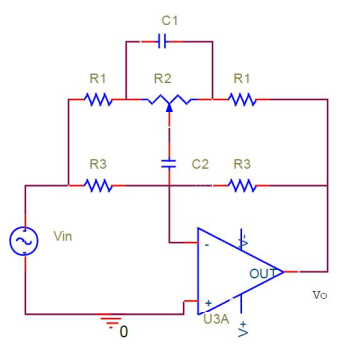
\includegraphics[scale=0.5]{Resources/Circuito}
\par\end{centering}
\caption{Circuito de Control de Tonos}
\label{5_1}

\end{figure}

\section{Transferencia}

Al calcular la transferencia genericamente para cualquier valor de
impedancias, y llamando a $R_{2}=R_{21}+R_{22}$, el calculo de la
transferencia se expresa como la ecuaci�n (\ref{eq:5_1}).

\[
H(s)=-\frac{C_{2}R_{3}s\left(R_{1}\left(C_{1}R_{2}s+1\right)-R_{2}\left(K-1\right)\right)\left(C_{1}R_{2}s+1\right)+C_{2}s\left(KR_{2}+R_{1}\left(C_{1}R_{2}s+1\right)\right)\left(R_{1}\left(C_{1}R_{2}s+1\right)-R_{2}\left(K-1\right)\right)+\left(-KR_{2}-2R_{1}\left(C_{1}R_{2}s+1\right)+R_{2}\left(K-1\right)\right)\left(C_{1}C_{2}KR_{2}^{2}s^{2}\left(K-1\right)-C_{1}R_{2}s-1\right)}{C_{2}R_{3}s\left(KR_{2}+R_{1}\left(C_{1}R_{2}s+1\right)\right)\left(C_{1}R_{2}s+1\right)+C_{2}s\left(KR_{2}+R_{1}\left(C_{1}R_{2}s+1\right)\right)\left(R_{1}\left(C_{1}R_{2}s+1\right)-R_{2}\left(K-1\right)\right)+\left(-KR_{2}-2R_{1}\left(C_{1}R_{2}s+1\right)+R_{2}\left(K-1\right)\right)\left(C_{1}C_{2}KR_{2}^{2}s^{2}\left(K-1\right)-C_{1}R_{2}s-1\right)}
\]

\[
H(s)=-\frac{20C_{2}^{2}K^{2}R_{1}R_{2}^{2}s^{2}-20C_{2}^{2}KR_{1}R_{2}^{2}s^{2}-10C_{2}^{2}R_{1}^{2}R_{2}s^{2}-100C_{2}^{2}R_{1}R_{2}^{2}s^{2}+C_{2}K^{2}R_{2}^{2}s+9C_{2}KR_{2}^{2}s-C_{2}R_{1}^{2}s-31C_{2}R_{1}R_{2}s-10C_{2}R_{2}^{2}s-2R_{1}-R_{2}}{20C_{2}^{2}K^{2}R_{1}R_{2}^{2}s^{2}-20C_{2}^{2}KR_{1}R_{2}^{2}s^{2}-10C_{2}^{2}R_{1}^{2}R_{2}s^{2}-100C_{2}^{2}R_{1}R_{2}^{2}s^{2}+C_{2}K^{2}R_{2}^{2}s-11C_{2}KR_{2}^{2}s-C_{2}R_{1}^{2}s-31C_{2}R_{1}R_{2}s-2R_{1}-R_{2}}
\]

\[
H(s)=-\frac{As^{2}+Bs+C}{Ds^{2}+Es+F}
\]

\[
A=20C_{2}^{2}K^{2}R_{1}R_{2}^{2}-20C_{2}^{2}KR_{1}R_{2}^{2}-10C_{2}^{2}R_{1}^{2}R_{2}-100C_{2}^{2}R_{1}R_{2}^{2}\approx-100C_{2}^{2}R_{1}R_{2}^{2}
\]

\[
B=C_{2}K^{2}R_{2}^{2}+9C_{2}KR_{2}^{2}-C_{2}R_{1}^{2}-31C_{2}R_{1}R_{2}-10C_{2}R_{2}^{2}
\]

\[
C=-2R_{1}-R_{2}
\]

\[
D=20C_{2}^{2}K^{2}R_{1}R_{2}^{2}-20C_{2}^{2}KR_{1}R_{2}^{2}-10C_{2}^{2}R_{1}^{2}R_{2}-100C_{2}^{2}R_{1}R_{2}^{2}=A
\]

\[
E=C_{2}K^{2}R_{2}^{2}-11C_{2}KR_{2}^{2}-C_{2}R_{1}^{2}-31C_{2}R_{1}R_{2}
\]

\[
F=-2R_{1}-R_{2}=C
\]

\[
\Rightarrow H(s)=-\frac{As^{2}+Bs+C}{As^{2}+Ds+C}
\]

\[
\frac{1}{\omega_{0}^{2}}=\frac{A}{C}
\]

\[
\Rightarrow\omega_{0}=\frac{\sqrt{2+\frac{R_{2}}{R_{1}}}}{10C_{2}R_{2}}\Longrightarrow f_{0}=\frac{\sqrt{2+\frac{R_{2}}{R_{1}}}}{20\pi C_{2}R_{2}}
\]

\[
Q_{z}=\frac{C}{B\omega_{0}}
\]

\[
Q_{z}=-\frac{10C_{2}\sqrt{R_{1}}R_{2}\sqrt{2R_{1}+R_{2}}}{C_{2}K^{2}R_{2}^{2}+9C_{2}KR_{2}^{2}-C_{2}R_{1}^{2}-31C_{2}R_{1}R_{2}-10C_{2}R_{2}^{2}}
\]

\[
Q_{p}=\frac{C}{E\omega_{0}}
\]

\[
Q_{p}=-\frac{10C_{2}\sqrt{R_{1}}R_{2}\sqrt{2R_{1}+R_{2}}}{-C_{2}K^{2}R_{2}^{2}+11C_{2}KR_{2}^{2}+C_{2}R_{1}^{2}+31C_{2}R_{1}R_{2}}
\]

\[
A=\frac{R_{1}^{2}+31R_{1}R_{2}+10R_{2}^{2}}{R_{1}\left(R_{1}+31R_{2}\right)}\approx\frac{3R_{1}+R_{2}}{3R_{1}}\,K=0
\]

\[
A=\frac{R_{1}\left(R_{1}+31R_{2}\right)}{R_{1}^{2}+31R_{1}R_{2}+10R_{2}^{2}}\approx\frac{3R_{1}}{R_{2}+3R_{1}}\,K=1
\]


\end{document}
